% 1977 年吉林卷第 1 题（3）：直角三角形 ABC，∠C 为直角（带直角标记），
% CD 为斜边 AB 上的高，D 在 AB 上（按源卷第 2 页布局：B 在上、C 左下、A 右下）
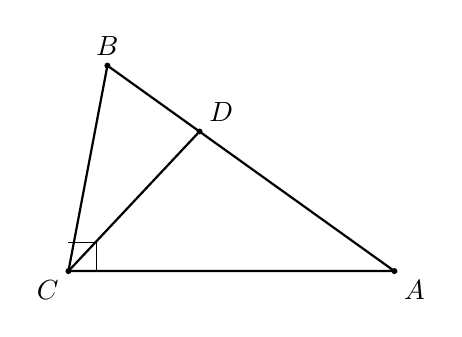
\begin{tikzpicture}[scale=0.9]
  \coordinate (C) at (0,0);
  \coordinate (A) at (4.6,0);
  \coordinate (B) at (0.55,2.9);
  \coordinate (D) at (1.85,1.97);
  \draw[thick] (A)--(B)--(C)--cycle;
  \draw[thick] (C)--(D);
  \draw (0.4,0) -- (0.4,0.4) -- (0,0.4);
  \fill (A) circle (1.2pt) node[below right] {$A$};
  \fill (B) circle (1.2pt) node[above] {$B$};
  \fill (C) circle (1.2pt) node[below left] {$C$};
  \fill (D) circle (1.2pt) node[above right] {$D$};
\end{tikzpicture}
